
\newcommand{\coef}{\textbf{c}}  
  
In this section we describe the implementation of the Chebyshev polynomial approximation to the Fermi distribution function. 
This is performed int the \texttt{~/qmd-progress/chebyshev\_mod.F90} module of the progress library. All the matrix-matrix multiplications are done with the BML library. 

The main objective of this technique is to approximate the following Fermi distribution function:
%
\begin{equation}
  f_F(\epsilon)= \frac{1}{1+\exp(\frac{\epsilon-\epsilon_F}{k_bT})}
  \label{Fermi}
\end{equation}
%
The electronic temperature $k_bT$ controls the derivative of this function when $\epsilon \simeq \epsilon_F$.
Here, $\epsilon_F$ is the Fermi level or electrochemical potential and $T$ is the temperatue.
%
\begin{equation}
  f'_F(\epsilon)= \frac{1}{k_bT}  
  \frac{-\exp{(\frac{\epsilon-\epsilon_F}{k_bT})}}{\left(1+\exp(\frac{\epsilon-\epsilon_F}{k_bT})\right)^2}
  \label{FermiD}
\end{equation}
%
When $\epsilon=\epsilon_F$: 
%
\begin{equation}
  f'_F(\epsilon)= -\frac{1}{4k_bT}  
  \label{FermiDEf}
\end{equation}
%
Hence, we can clearly see that, when the temperature is increased, the derivative of the Fermi funtion, at $\epsilon=\epsilon_F$, decreases in absolute value.  

For very small temperatures (300 K for example), this function can be considered as a step function. In other words, if $k_bT \simeq 0.0$, then:
%
\begin{equation}
  f_F(\epsilon) = \left\{\begin{array}{clrr}
    1.0, & \mathrm{if} \quad  \epsilon < \epsilon_F \\
    1/2, &  \mathrm{if}  \quad  \epsilon = \epsilon_F \\
    0.0, &  \mathrm{if}  \quad  \epsilon >\epsilon_F
  \end{array}\right.
  \label{adj}
\end{equation}

\subsection{Chebyshev polynomial properties}

The formal definition of these polynomial is the following: The nth Chebyshev polynomial is defined as follows: 
%
\begin{equation}
  T_n(x)= \cos\left[n \cos^{-1}(x) \right]
  \label{nthcheb}
\end{equation}

With $x \in [-1,1]$ and $n \in 0,1,2, ...$

These polynomial follow a special recurence relation: 
%
\begin{equation}
  T_{n+1}(x)= 2xT_{n}(x) - T_{n-1}(x)
  \label{recursion}
\end{equation}
%
With $T_0 = 1$ and $T_1 = x$.
This can be easilly proven by explicitly writting the definitions at both sides of the equality of equation \ref{recursion} 
Another important property is that, $T_n(x)$ has $n$ zeroes lying in the interval $(-1,1)$. These zeroes are given by: 

\begin{equation}
  x_k = \cos\left(\frac{2k+1}{2n}\pi\right), \, k=0,1,...,n-1
  \label{zeroes}
\end{equation}


One of the most useful property is the orthogonality relation:

\begin{equation}
  \int_{-1}^{1}{ T_r(x) T_s(x) (1-x^2)^{-1/2}} dx = N_r\delta_{rs} 
  \label{zeroes}
\end{equation}

Which has a discrete version that uses the zeros as nodes as follows:

\begin{equation}
  \braket{T_r}{T_s} =  \sum_{j=0}^{n}{T_r(x_j) T_s(x_j)}= K_r\delta_{rs} 
  \label{zeroes}
\end{equation}

Where $K_0 = n + 1$ and $K_r = (n + 1)/2$ for $1 \leq r \leq n$. Note that $(1-x^2)^{-1/2}$ in $x_k$


\subsection{Fermi function approximation}

Here we use this orthogonality relation to compute the coefficient of the Chebyshev polynimial to approximate the Fermi distribution function as follows:

\begin{equation}
  f_F(x) \simeq f^m_F(x) = \sum_i^m c_i T_i(x)
\end{equation}

where $c_i$ are the coefficients of the expansion and $T_i(x)$ as the Chebyshev polynomial.
We can notice that: $f^0_F(x) = c_0$ and $f^1_F(x) = c_1x + c_0$ and applying the recursive relation we have: 

\begin{equation}
  f^{m+1}_F(x) = f^m_F(x) + c_{n+1}T_{n+1}
\end{equation}

This means that, if we know the coefficients up to $m$ we can construct the approximations applying the following steps of recursion: 

\begin{equation}
  \begin{array}{ccc}    
    T_{n+1}(x) = 2xT_n(x) - T_{n-1}(x)  \\
    f^{m+1}_F(x) = f^m_F(x) + c_{n+1}T_{n+1}
  \end{array}    
\end{equation}
For all the points $x$ in the domain and taking into account that $T_0 = 1$, $T_1=x$, $f^0_F(x) = c_0$ and $f^1_F(x) = c_1x + c_0$.

We know that $\braket{f_F}{T_r} = c_r$ since: 

\begin{equation}
  \braket{f_F}{T_r} \simeq \sum_i^m c_i \braket{T_i}{T_r} = c_r
\end{equation}

And we also know that the domain of the function has to be constrain to $[-1,1]$. For this purpose, we apply the following transformation:
\begin{equation}
  \tilde{x} = \frac{2(x-x_{min})} {(x_{max}-x_{min})} - 1
\end{equation}

and 

\begin{equation}
  x = \frac{(\tilde{x} + 1)(x_{max}-x_{min})}{2}  + x_{min}
  \label{x}
\end{equation}


Where $x_{max}$ and $x_{min}$ are estimations of the domain boundaries of $f$ and for our case we could use the Girshgorin circle theorem. And the same transformation can be applied to the Hamiltonian matrix in our case: 
\begin{equation}
  \tilde{H} = \alpha H  +  \beta I
\end{equation}

Where $H$ is the Hamiltonian matrix and $I$ is the identity matrix. $\alpha$ and $\beta$ are defined as follows: 

\begin{equation}
  \begin{array}{ccc}    
  \alpha = \frac{2}{(x_{max}-x_{min})} \\
  \beta = - \frac{2x_{min}}{(x_{max}-x_{min})} - 1
  \end{array}
\end{equation}

The function $f_F$, also have to get arguments in $[-1,1]$ for which we have to do: 

\begin{equation}
  \tilde{f}_F(\tilde{x})= \frac{1}{1+\exp(\frac{(\frac{\tilde{x} - \beta}{\alpha})-x_F}{k_bT})}
  \label{Fermi}
\end{equation}

Our fist attempt for an pseudocode would look like the following: 

Derivative AS A FUINCTION OF MOMENTS!!!HOW DOES IT CHANGES 

\begin{algorithm}[H]
  \algrenewcommand\algorithmicfunction{\textbf{procedure}}
  \begin{algorithmic}
    \parskip 0.05cm
    {\fontsize{0.3cm}{0.3em}\selectfont 
      \Function{CHEB}{$m$, $k_bT$, $\mu$, $\ham$, $\pno$}
      %
      \State Estimate $\emin$ and $\emax$ from $\ham$
      %
      \State Compute $\alpha$ and $\beta$      
      %
      \State $\X = \alpha\ham + \beta \Id$
      %
      \State \textbf{call} \textcolor{blue}{GETC}($k_bT,\mu,m,\alpha,\beta,\coef$) 
      %
      \State $\textbf{T}_0 = \Id$; $\textbf{T}_1 = \X$
      \State $\X_0 = c_0\Id$; $\X_1 = \X_0 + c_1\textbf{T}_1 $
      \State \textbf{for} $j$ = 1 : $m-1$ \textbf{do}
      
      \State \qquad \textcolor{red}{$\textbf{T} = 2\X\textbf{T}_1 - \textbf{T}_{0}$}
      \State \qquad $\X = \X_1 + c_{n+1}\textbf{T}$
      \State \qquad $\X_1 = \X$; $\textbf{T}_{0} = \textbf{T}_{1}$; $\textbf{T}_{1} = \textbf{T}$  
      \State \textbf{end for}
      %
      \State $\pno = \X$
      %     
      \EndFunction
    }       
  \end{algorithmic}
  \label{pcode}
  \caption{Pseudocode for the Chebyshev kernel polynomial method.}
\end{algorithm}

\begin{algorithm}[H]
  \algrenewcommand\algorithmicfunction{\textbf{procedure}}
  \begin{algorithmic}
    \parskip 0.05cm
    {\fontsize{0.3cm}{0.3em}\selectfont 
      \Function{GETC}{$k_bT$,$\mu$,$m$,$\alpha$,$\beta$,$\coef$}
      %
      \State \textbf{for} $r$ = 1 : $m - 1$ \textbf{do}\\
      \State \qquad \textbf{for} $j$ = 1 : $n$ \textbf{do}        
      \State \qquad \qquad $x_j = \cos((j+0.5)\pi/(n + 1))$
      \State \qquad \qquad $x = \frac{x_j - \beta}{\alpha}$
      \State \qquad \qquad $Int = Int + T_r(x_j)\mathrm{Fermi}(x,\mu,k_bT)$            
      \State \qquad \textbf{end for}        \\
      \State \qquad \textbf{if}($r = 0$) \textbf{then}
      \State \qquad \qquad $c_{r+1} = Int/K_0$
      \State \qquad \textbf{else}      
      \State \qquad \qquad $c_{r+1} = Int/K_r$
      \State \qquad \textbf{end if}           \\ 
      \State \textbf{end for}
      %
      \EndFunction
    }       
  \end{algorithmic}
  \label{pcode}
  \caption{Pseudocode for computing the Chebyshev coefficients}
\end{algorithm}

% \State \textbf{for} $r$ = 1 : $m - 1$ \textbf{do}
% \State \qquad \textbf{for} $j$ = 1 : 1000 \textbf{do}        
% \State \qquad \qquad xj = cos((j+0.5_dp)*pi/(npts + 1))
% \State \qquad \qquad x = (emax-emin)*(xj + 1.0d0)/2.0d0 + emin
% \State \qquad \qquad Int = Int + Tr(r,xj)*fermi(x,ef,kbt)      
% \State\qquad \textbf{end for}  

The Jacson kernel gives un a higher temperatue. The problem is that we miss accuracy around the Fermi level. 

\begin{itemize}
 \item Hybrid between SP2 and Cheb expansion. We tried performing Cheb first followed by SP2 and viceversa. There's no imporvement 
 compared to ``truncated'' SP2. 
 
\end{itemize}


Chebyshev polynomial approximation to the Fermi distribution. Some points:
\begin{itemize}
 \item Trivial parallelization and the possibility of using sparse Matrix-Matrix multiplications (BML)
 \item Potential use of common kernel that will be developed in COPA for SP2 and SP2\_Fermi
 \item Requires several matrix-matrix multiplications depending on the electronic T.  
\end{itemize}

  \begin{itemize}
   \item     - Alexander Weisse, Gerhard Wellein, Andreas Alvermann, and Holger Fehske. The kernel polynomial method. \textit{Rev. Mod. Phys.}, 78:275-306, \textbf{2006}. 
  \item     - Javier Segura Amparo Gil and Nico M. Temme. Chebyshev Expansions, chapter 3. \textit{Society for Industrial Mathematics (SIAM)}, \textbf{2007}.
  \item - R. N. Silver, H. Roeder, A. F. Voter, and J. D. Kress. Chebyshev Moment Problems: Maximum Entropy and Kernel Polynomial Methods, pages 187–194. \textit{Springer} Netherlands, Dordrecht, \textbf{1996}. 
  \end{itemize}  
  


The Fermi distribution function can be approximated with Chebyshev polynomials: 
\begin{equation}
  f_F(\epsilon)= \frac{1}{1+\exp(\frac{\epsilon-\epsilon_F}{k_bT})}
  \label{Fermi}
\end{equation}
\vspace{0.3cm}
\begin{equation}
  f_F(x) \simeq f^m_F(x) = \sum_i^m c_i T_i(x)
\end{equation}
where $c_i$ are the coefficients of the expansion and $T_i(x)$ are the Chebyshev polynomial.
  \footnote{\tiny
    - Alexander Weisse, Gerhard Wellein, Andreas Alvermann, and Holger Fehske. The kernel polynomial method. \textit{Rev. Mod. Phys.}, 78:275-306, \textbf{2006}. 
  }


  This means that, if we know the coefficients up to $m$ we can construct the approximation applying the following steps of recursion: 
\begin{equation}
    T_{n+1}(x) = 2xT_n(x) - T_{n-1}(x) 
\end{equation}
\begin{equation}
    f^{m+1}_F(x) = f^m_F(x) + c_{n+1}T_{n+1}
\end{equation}
For all the points $x$ in the domain and taking into account that $T_0 = 1$, $T_1=x$, $f^0_F(x) = c_0$ and $f^1_F(x) = c_1x + c_0$. \\
\vspace{0.4cm}
Note that $x$ can be a Hamiltonian matrix $\textbf{H}$.
  \footnote{\tiny
    - Alexander Weisse, Gerhard Wellein, Andreas Alvermann, and Holger Fehske. The kernel polynomial method. \textit{Rev. Mod. Phys.}, 78:275-306, \textbf{2006}. 
  }


Fermi function evaluated and approximated over the 50 CH$_4$ system spectral domain:
   \begin{center}
    \begin{tikzpicture}
      \node (a) [xshift=0.0cm,yshift=0.0cm] {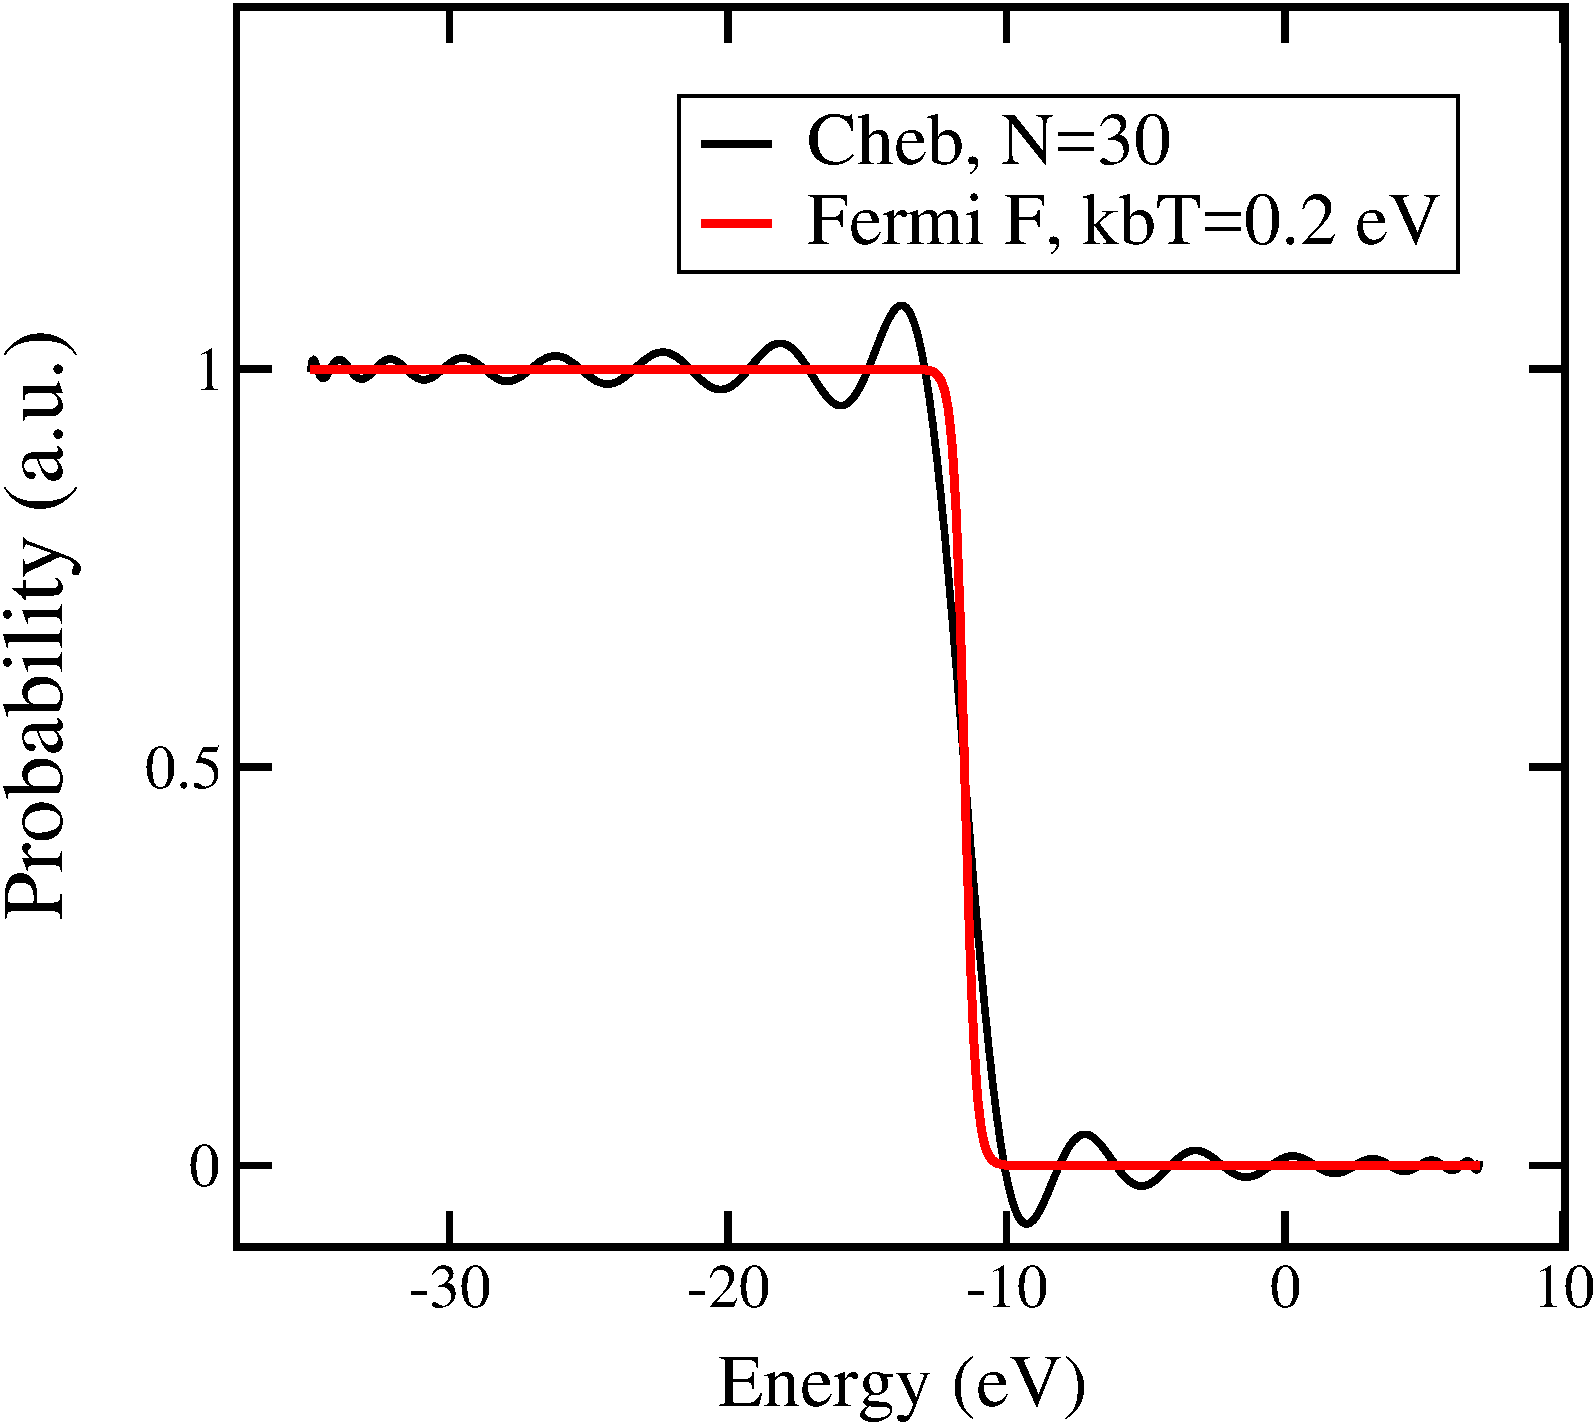
\includegraphics[width=6.0cm]{./fig/30.pdf}};          
    \end{tikzpicture}
   \end{center}  
We can note that the ``Gibbs oscillations'' that are definitely a problem for electronic structure calculations. 


Any kind of oscillations can give problems when computing the total occupation.
   \begin{center}
    \begin{tikzpicture}
      \node (a) [xshift=0.0cm,yshift=0.0cm] {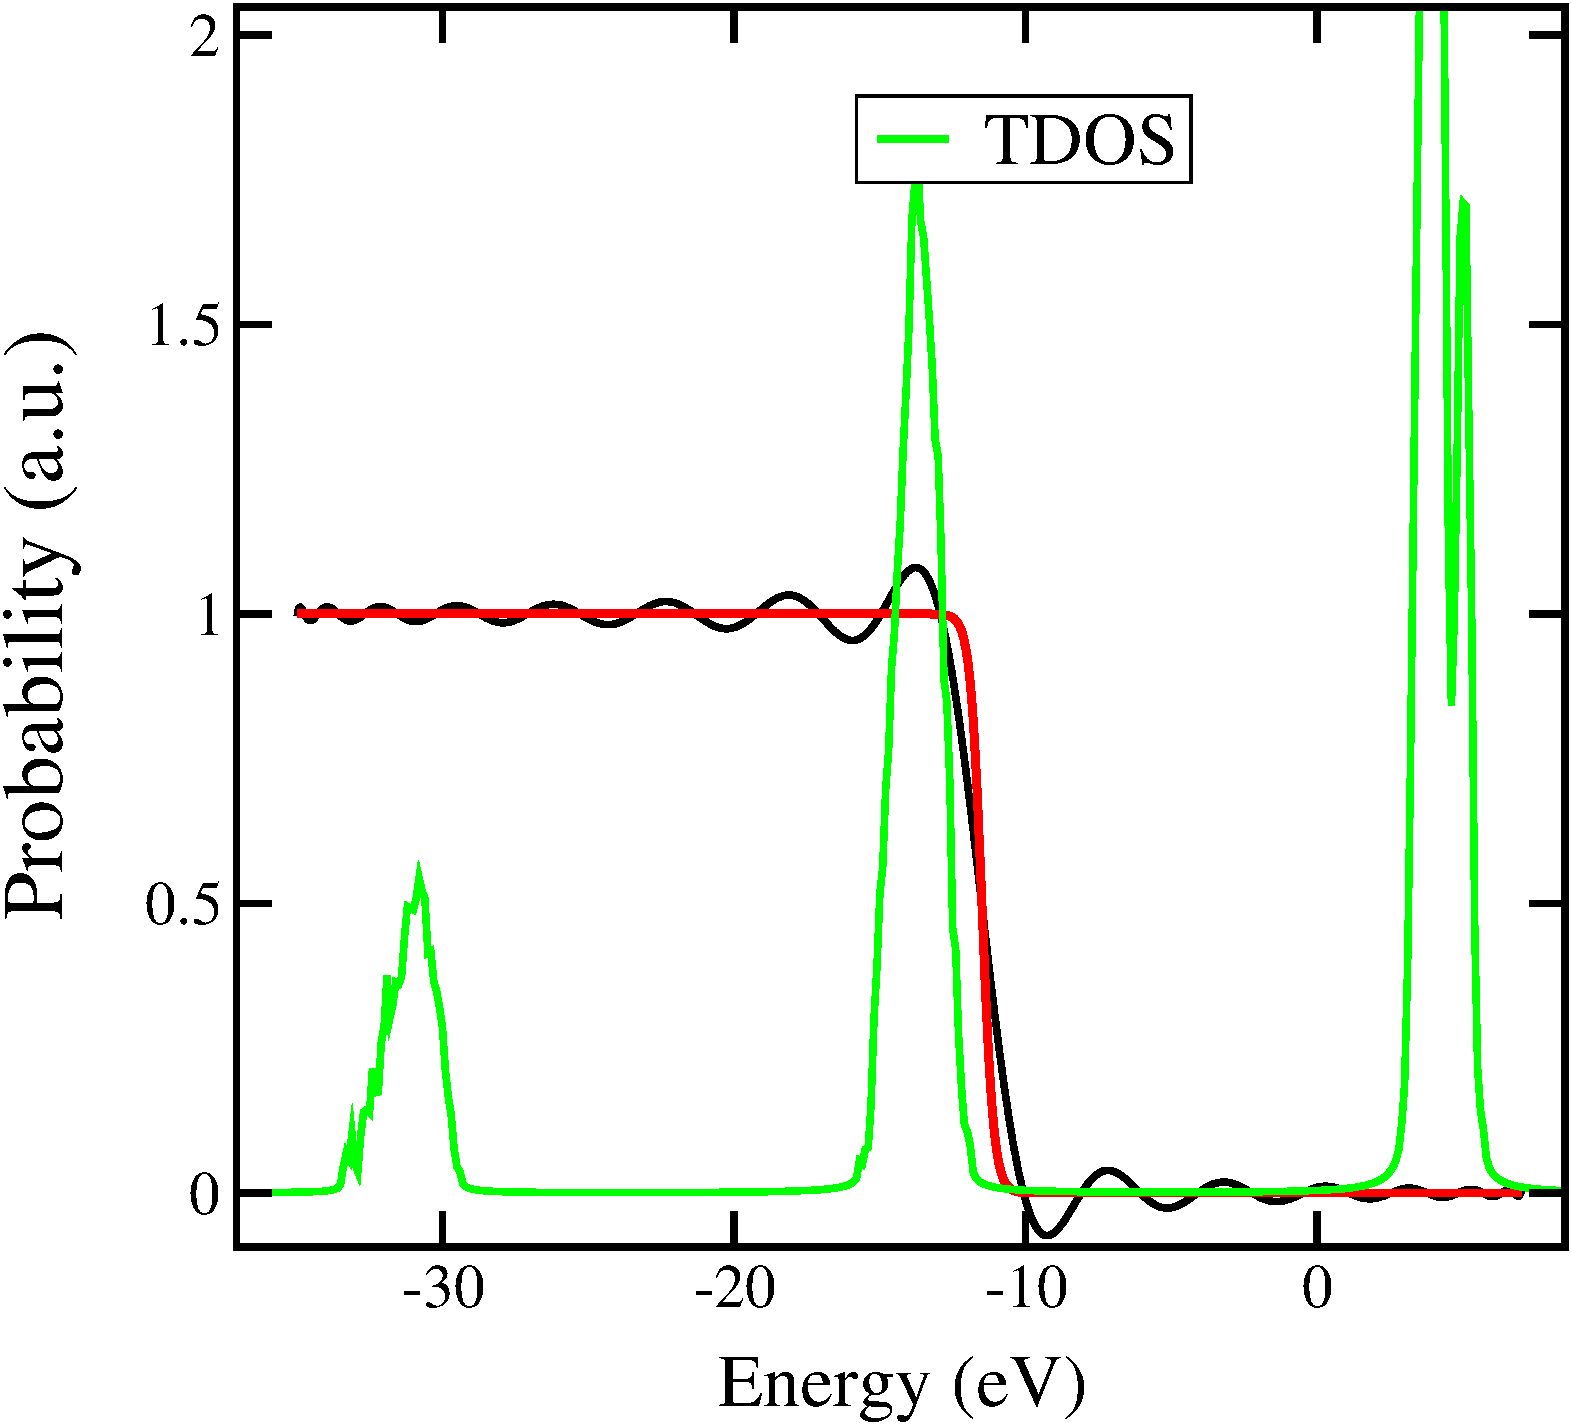
\includegraphics[width=6.0cm]{./fig/tdoscomp.pdf}};          
    \end{tikzpicture}
   \end{center}  
Oscillations around zones with ``rich states'' cause problems.



It can be corrected by applying the Jackson kernel. But with disadvantage of having a lower derivative at $x = \mu$.
\begin{equation}
       g^J_i = \frac{1}{n+1} (n - i + 1) \cos \frac{\pi i}{n+1} 
             +   \sin \frac{\pi i}{n+1} \cot \frac{\pi}{n+1}
\end{equation}
   \begin{center}
    \begin{tikzpicture}
      \node (a) [xshift=0.0cm,yshift=0.0cm] {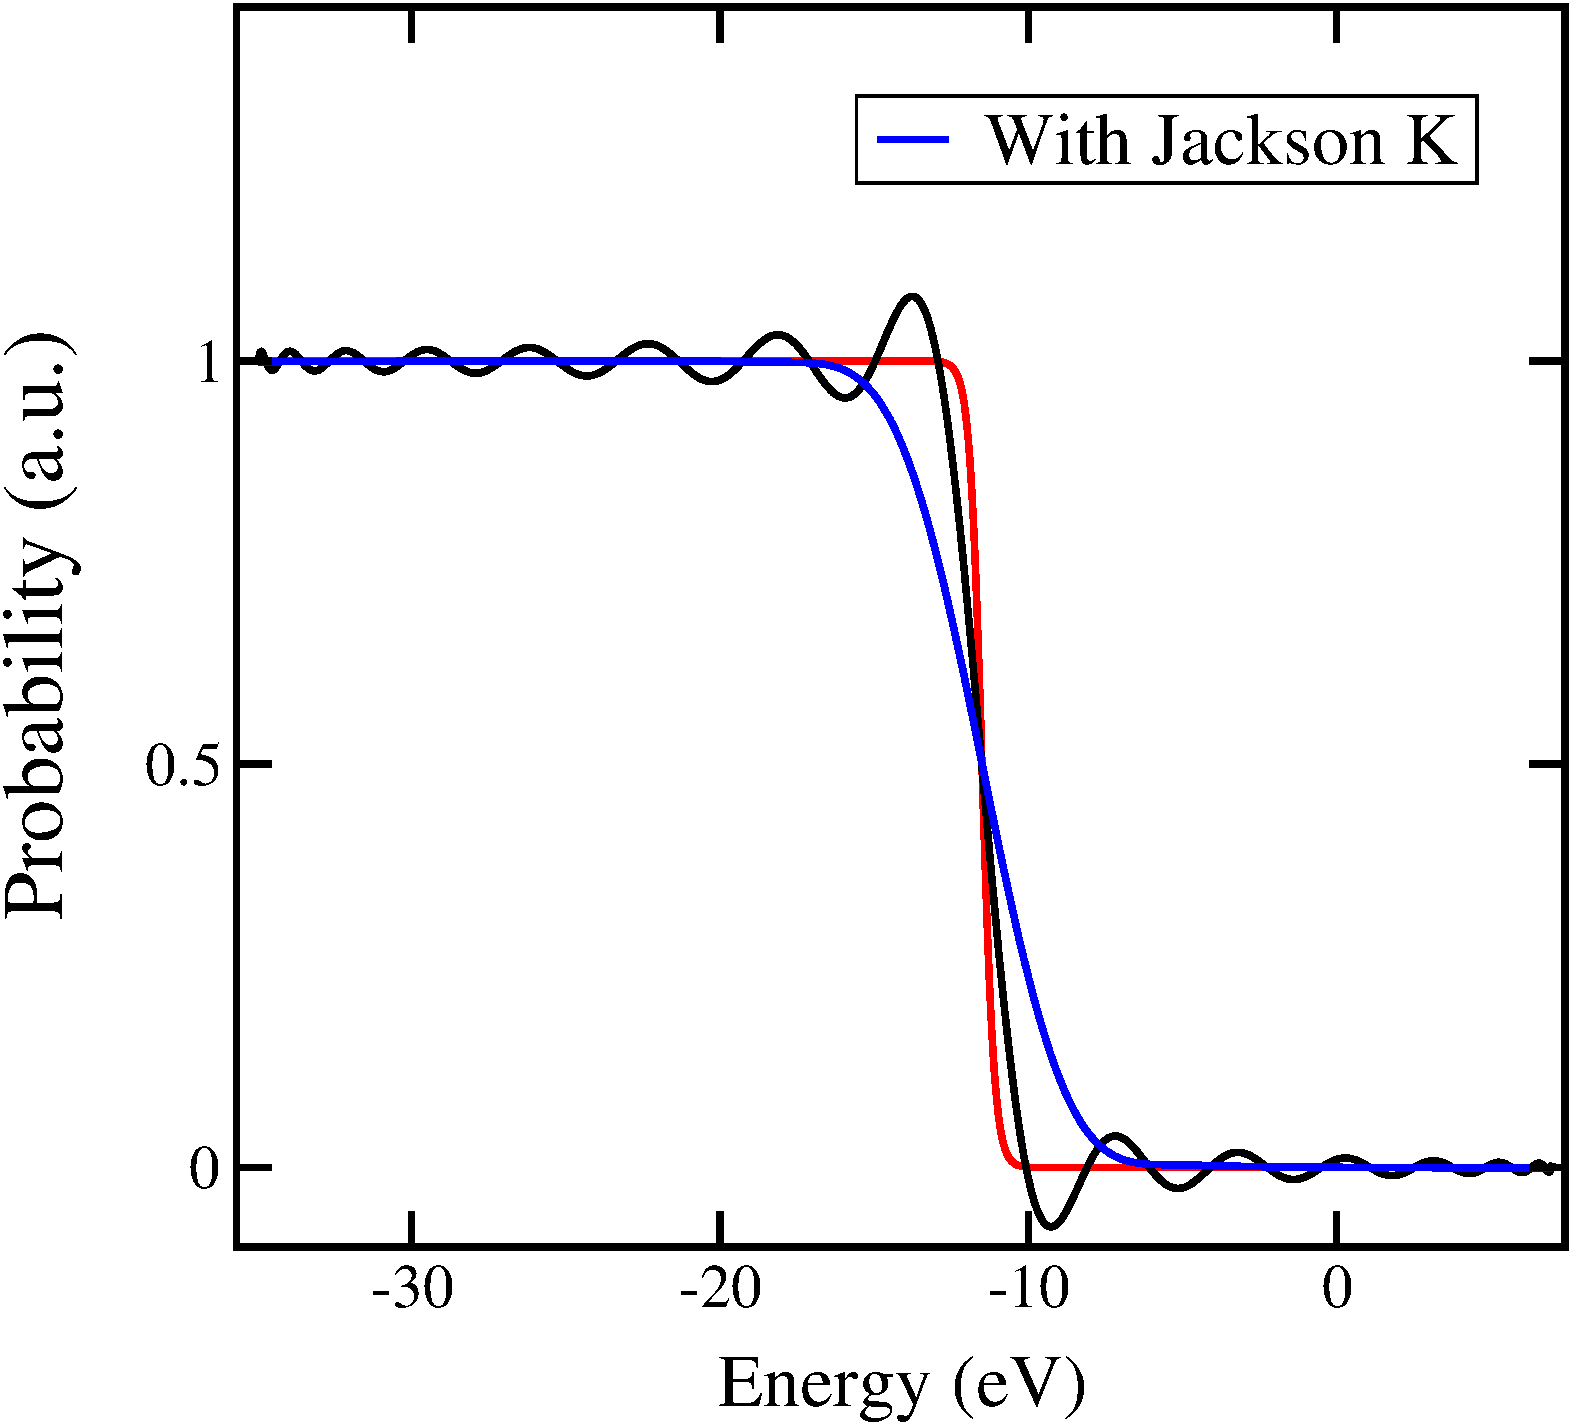
\includegraphics[width=6.0cm]{./fig/jac.pdf}};          
    \end{tikzpicture}
   \end{center}  

Gap resolution as a function of the number of polynomials for the 50 CH$_4$ system.
   \begin{center}
    \begin{tikzpicture}
      \node (a) [xshift=0.0cm,yshift=0.0cm] {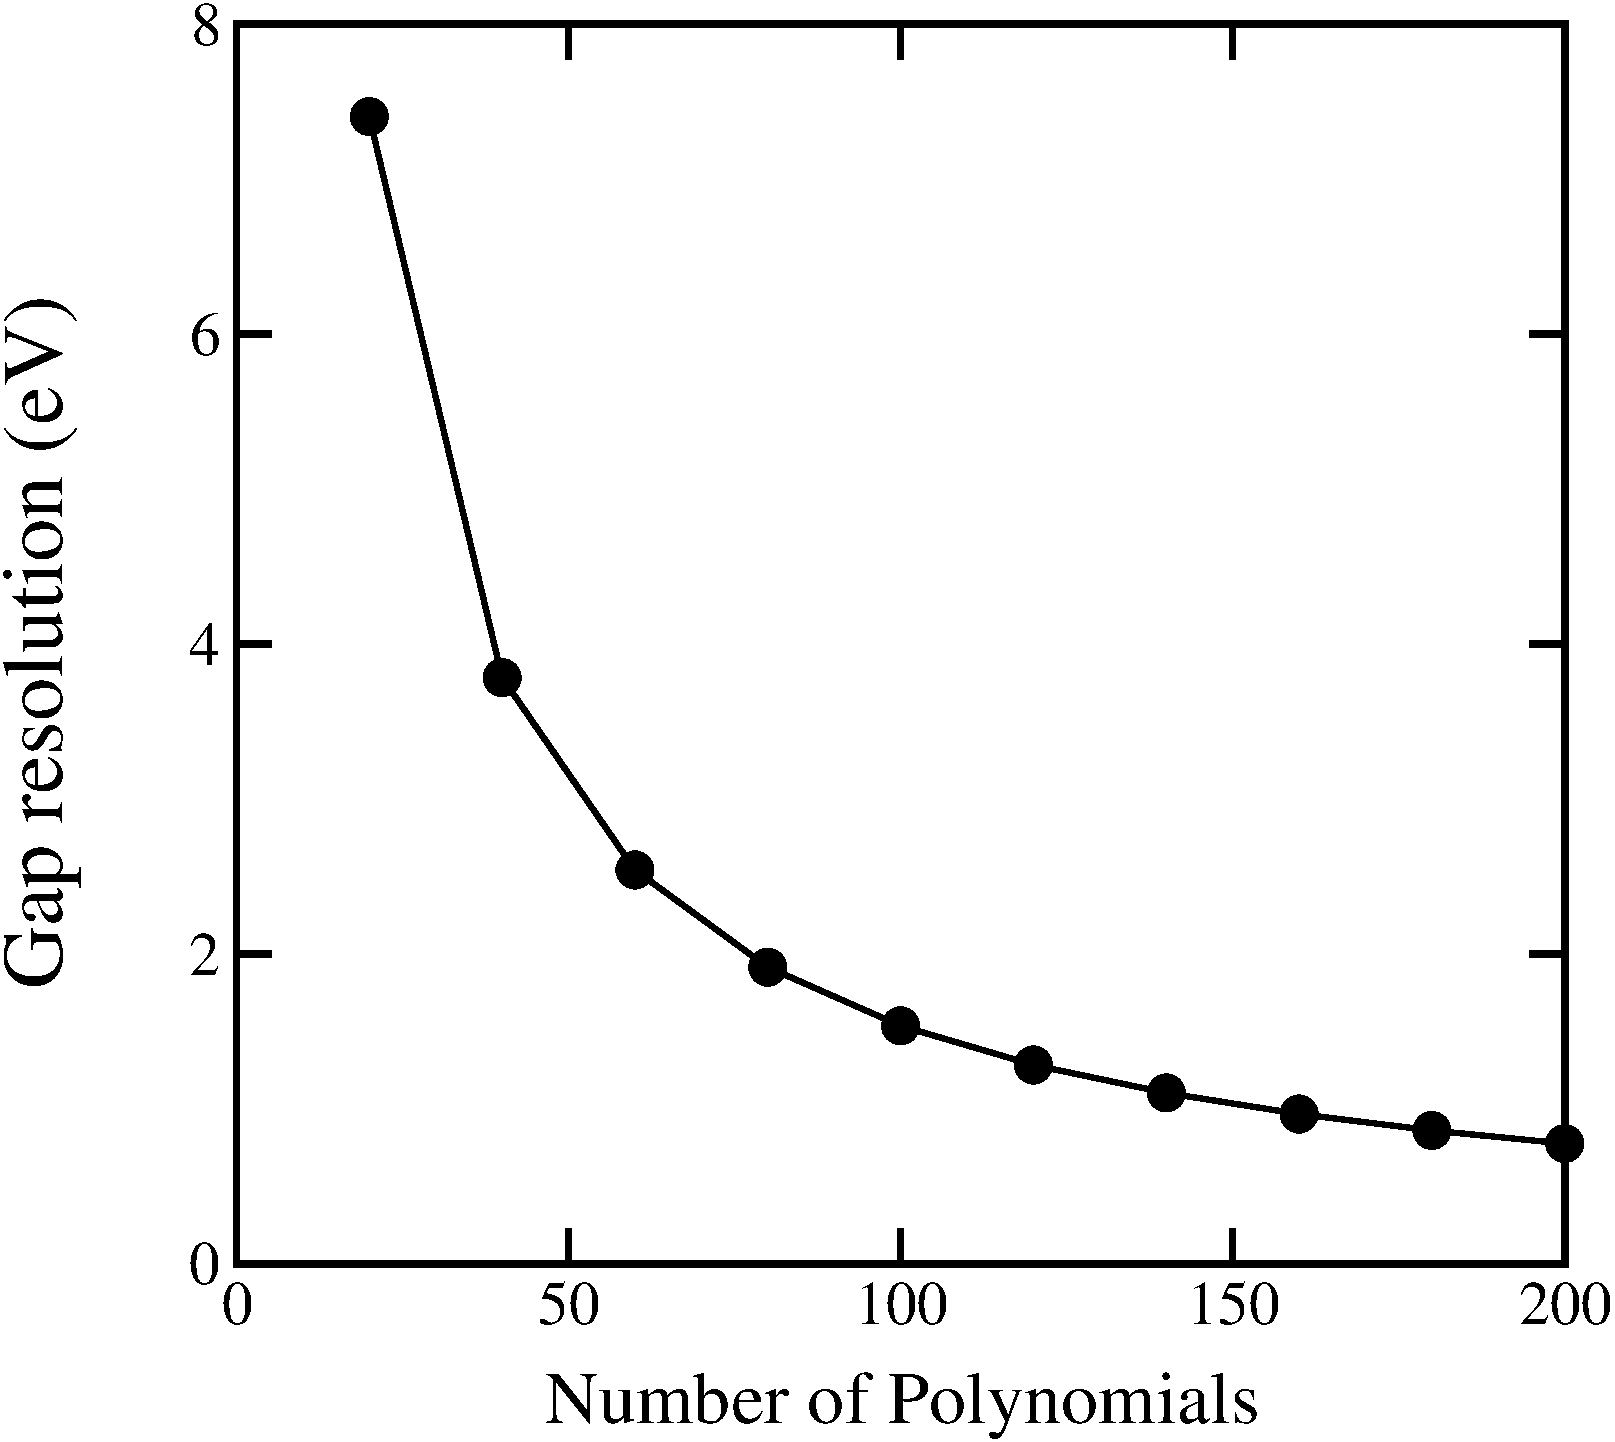
\includegraphics[width=6.0cm]{./fig/gap.pdf}};          
    \end{tikzpicture}
   \end{center}  


\begin{algorithm}[H]
  \algrenewcommand\algorithmicfunction{\textbf{procedure}}
  \begin{algorithmic}
    \parskip 0.05cm
    {\fontsize{0.3cm}{0.3em}\selectfont 
      \Function{CHEB}{$m$, $k_bT$, $\mu$, $\bold H$, $ \bold P$}
      %
      \State Estimate $\emin$ and $\emax$ from $\ham$
      %
      \State Compute $\alpha$ and $\beta$      
      %
      \State $\X = \alpha\ham + \beta \Id$
      %
      \State \textbf{call} \textcolor{blue}{GETC} ($k_bT,\mu,m,\alpha,\beta,\coef$) 
      %
      \State $\textbf{T}_0 = \Id$; $\textbf{T}_1 = \X$
      \State $\X_0 = c_0\Id$; $\X_1 = \X_0 + c_1\textbf{T}_1 $
      \State \textbf{for} $j$ = 1 : $m-1$ \textbf{do}
      
      \State \qquad \textcolor{red}{$\textbf{T} = 2\X\textbf{T}_1 - \textbf{T}_{0}$}
      \State \qquad $\X = \X_1 + c_{n+1}\textbf{T}$
      \State \qquad $\X_1 = \X$; $\textbf{T}_{0} = \textbf{T}_{1}$; $\textbf{T}_{1} = \textbf{T}$  
      \State \textbf{end for}
      %
      \State $\pno = \X$
      %     
      \EndFunction
    }       
  \end{algorithmic}
  \label{pcode}
  \caption{Pseudocode for the Chebyshev kernel polynomial method.}
\end{algorithm}
All the operations are done with the BML library. Function GETC, gets the coefficients of the expansion. 



Things we tried:
\begin{itemize}
 \item Hybrid Chebyshev and SP2 methods. 
 \item SP2 $\longmapsto$ Cheb. We get Gibbs oscillations but the Fermi function is well approximated.
 \item Cheb $\longmapsto$ SP2. Same as the ``truncated'' SP2 (No benefit from Cheb expansion).
 \item SP2 $\longmapsto$ Cheb $\longmapsto$ SP2 $\longmapsto$. We get Gibbs osculations.   
\end{itemize}
Things to do:
\begin{itemize}
 \item Better estimation of the spectral boundaries with the power method.
 \item Tests the scaling with sparse matrix-matrix algebra. 
 \item Compare efficiency with SP2.
 \item Add matrix-(rectangular matrix) multiplications at BML level.
\end{itemize}

We propose to have a linear function of the threshold, increasing linearly with the degree. 

\begin{equation}
   \mathrm{thr}(n) = \mathrm{thr_0}(a(n-1)+1)
\end{equation}
\\
\vspace{0.5cm}
This function ensures $\mathrm{thr}(1) = \mathrm{thr_0}$

\vspace{0.5cm}

The error in the approximation if estimated as: 

\begin{equation}
   Error = \frac{Fn(\rho_{\mathrm{Cheb}} - \rho_{\mathrm{Exact}})}{N}
\end{equation}

\vspace{0.5cm}

Where $\rho_{\mathrm{Exact}} = C f(e) C^T$

We have plotted the scaling for different values of parameter $a$.

   \begin{center}
    \begin{tikzpicture}
      \node (a) [xshift=0.0cm,yshift=0.0cm] {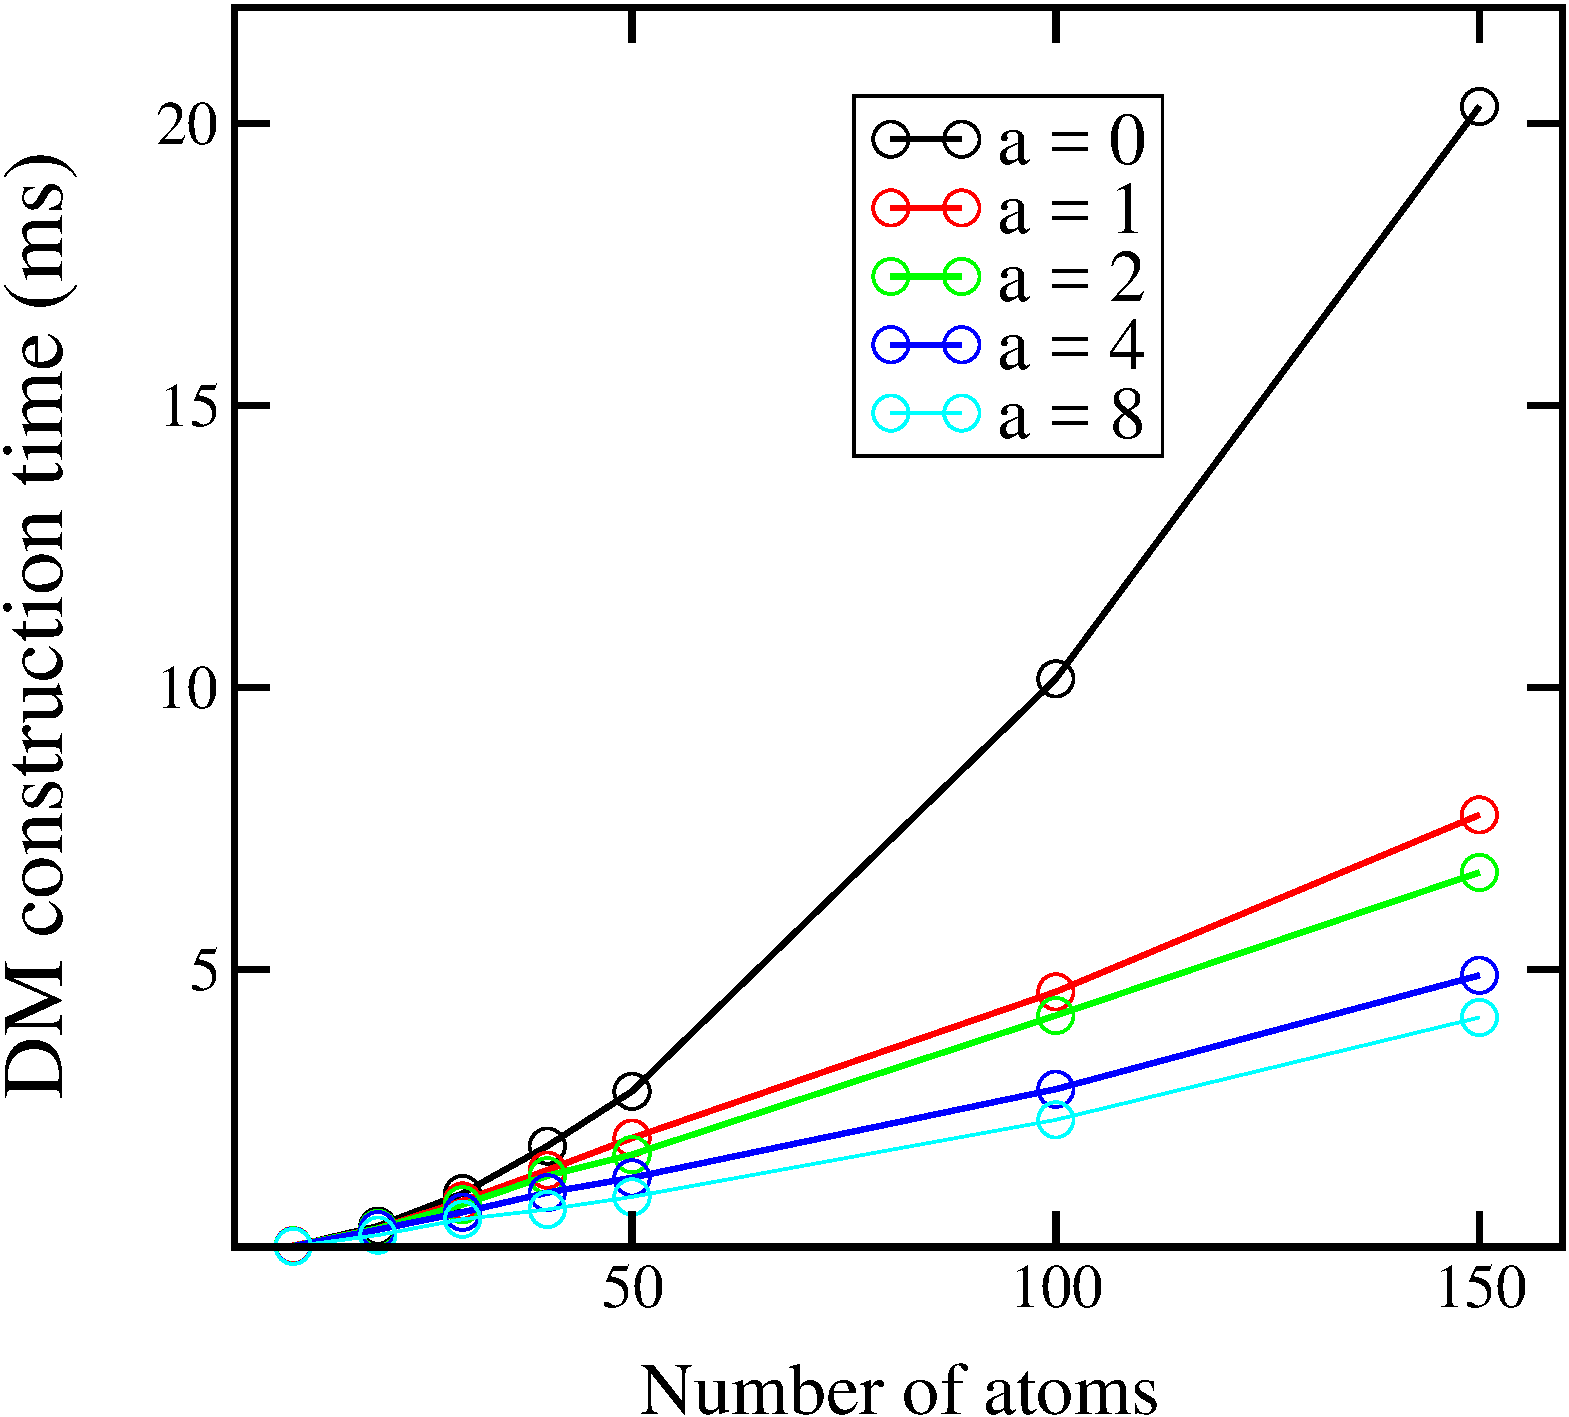
\includegraphics[width=6.0cm]{./fig/time_a_parameter.pdf}};          
    \end{tikzpicture}
   \end{center}  



We have plotted the scaling for different values of parameter $a$.

   \begin{center}
    \begin{tikzpicture}
      \node (a) [xshift=0.0cm,yshift=0.0cm] {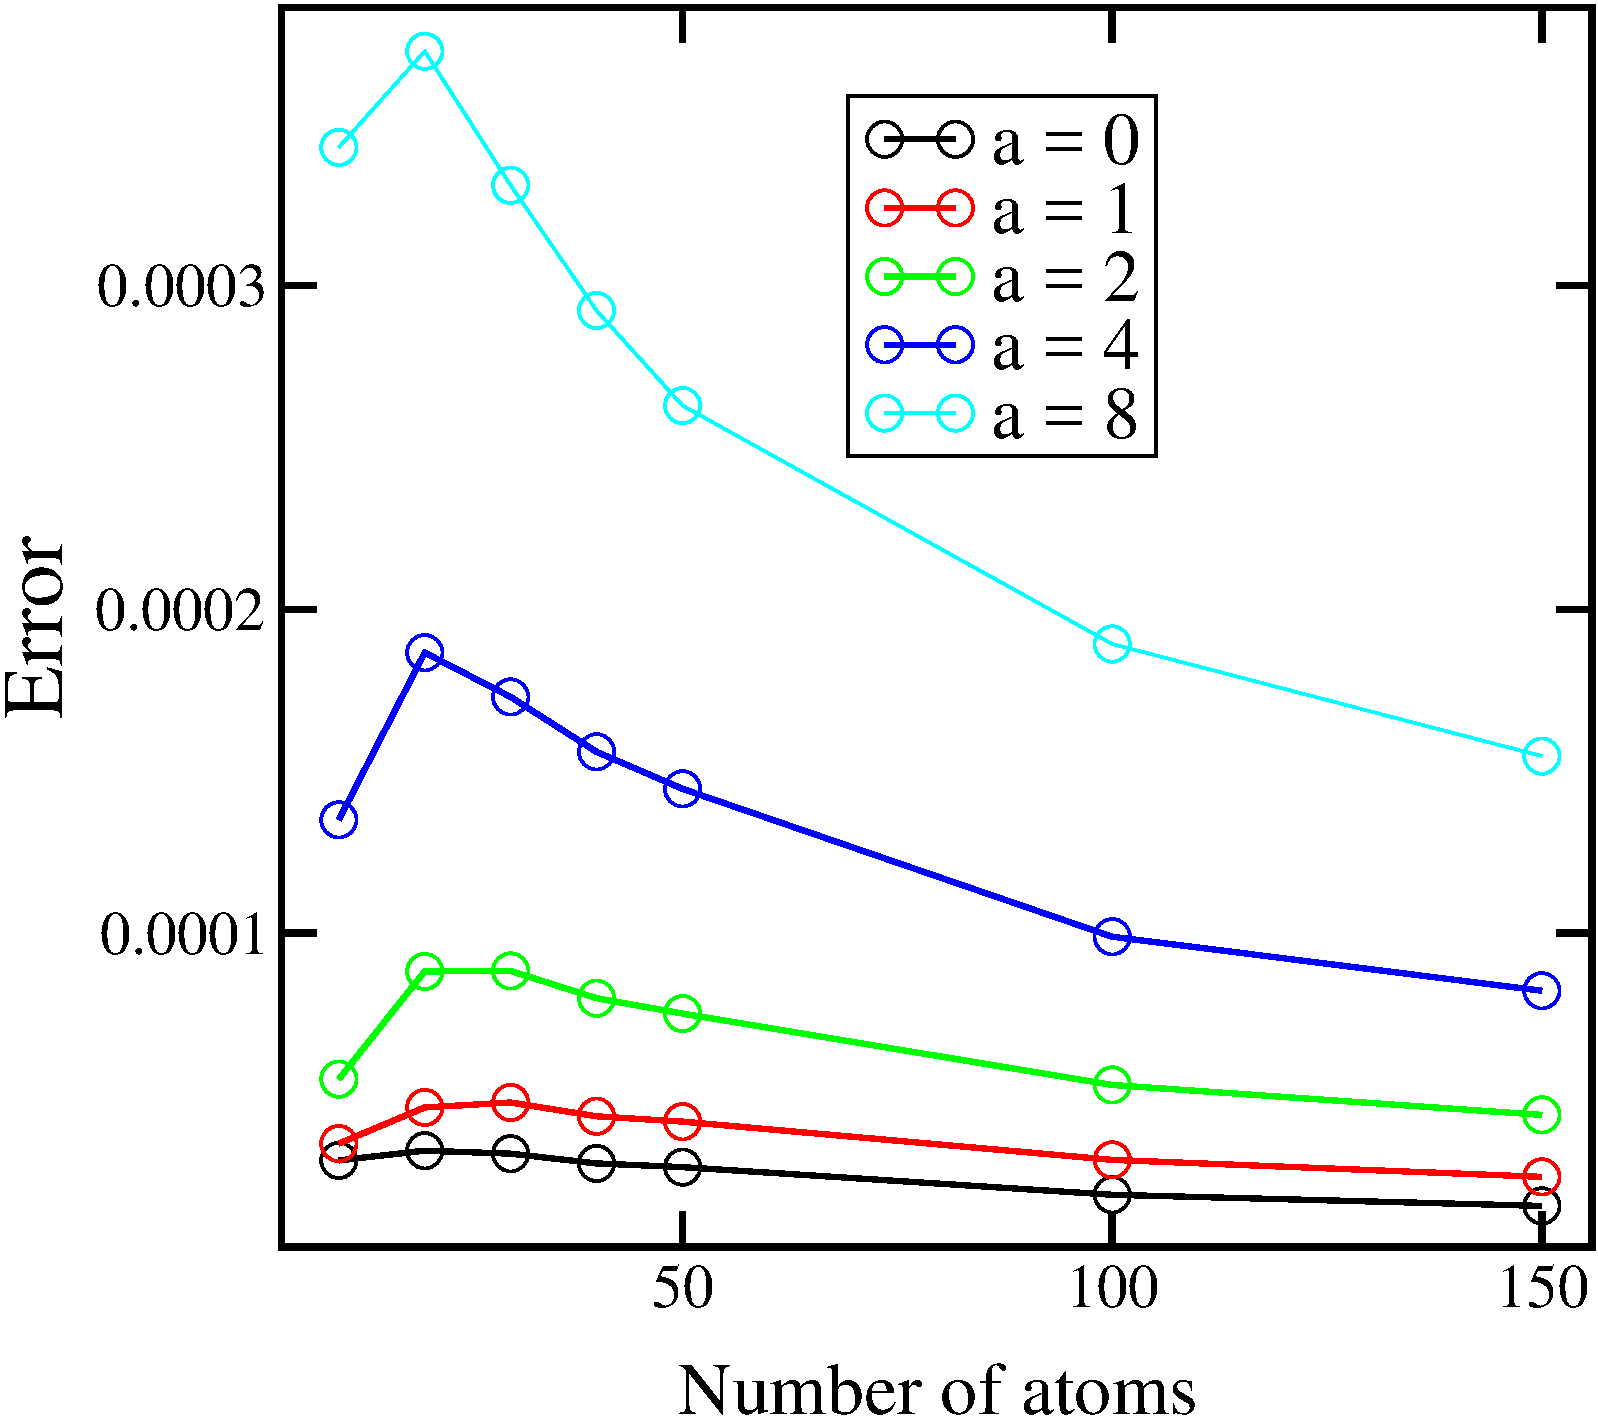
\includegraphics[width=6.0cm]{./fig/error_a_parameter.pdf}};          
    \end{tikzpicture}
   \end{center}  



